\chapter{Blockchains with Finality}
\section{Review of the longest chain protocol}
The longest chain consensus protocol was the main idea of focus and concentration in the previous chapters. This protocol and its modifications we have seen so far, all favor liveness, but are not safe under network partition.\\
The protocol has some advantages and disadvantages in terms of liveness and safety :
\begin{itemize}
	\item \textbf{Liveness} : \\
	the protocol is live even with minuscule honest hash power. Even a single honest miner with a small hash power can extend the longest chain.
	\item \textbf{Safety} : \\
	The protocol only guarantees safety when the hash power of honest nodes is more than 50\% but with two caveats:
	\begin{enumerate}
		\item \textbf{Probabilistic guarantee} :
		The safety of the confirmed blocks is provided in terms of the probability of deconfirmation ("error").
		\item \textbf{Network must be synchronous} :
		Honest nodes need to update each other regularly on the status of the longest chain, so that they can work together on extending the same chain, avoiding splitting.
	\end{enumerate}
\end{itemize}
In some applications, safety is very important, especially deterministic guarantees (known as \textbf{"finality"}) for a confirmed ledger entry, e.g., financial applications. The longest chain protocol (and any of the variations we saw in the previous chapters) cannot provide much relief in this case.
\begin{figure}[h!]
	\centering
	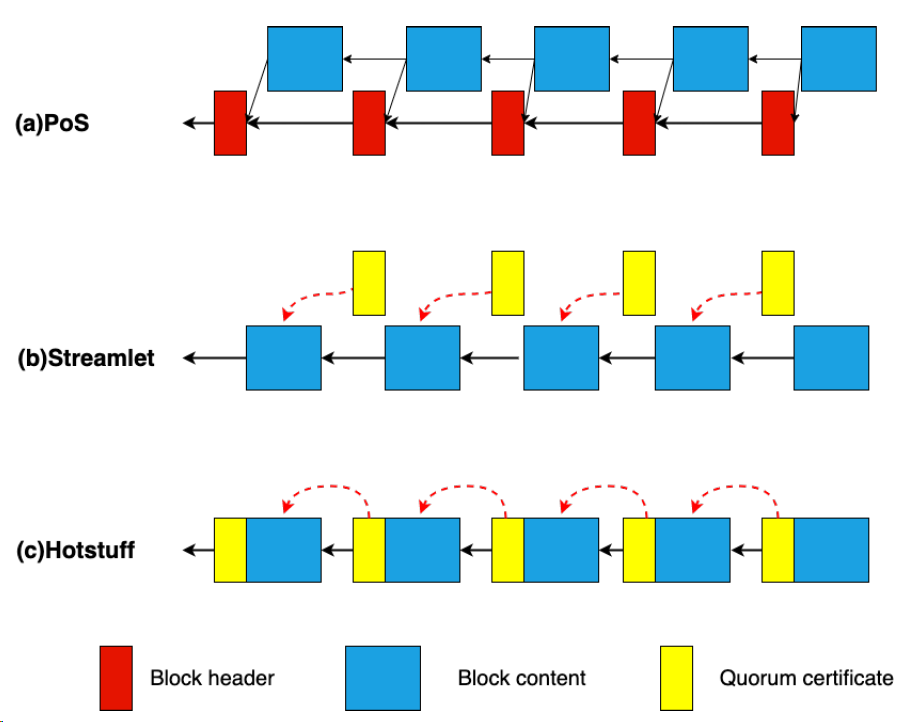
\includegraphics[width=0.5\linewidth]{Fig/15/F8}
	\caption{}
	\label{fig:L15_f8}
\end{figure}


\section{Byzantine Fault Tolerant (BFT) Protocols}
Byzantine Fault Tolerant (BFT) Protocols are a class of blockchain protocols that can achieve deterministic safety even under the asynchronous network conditions. This means that they can guarantee that the confirmed ledger entries are final and unchangeable, even if some nodes are malicious or the network is slow or unreliable. Two closely related protocols that belong to this class are \textbf{Streamlet and HotStuff}.\\\\
The BFT protocol works with a set of nodes (called $N$) that are fixed and have a fixed identity (public key) that everyone knows.
The protocol runs in rounds, which are numbered by integers, similar to the PoS longest chain protocols. But unlike the PoS protocols, here only one proposer is picked in each round. The proposer has to be chosen and checked in a distributed way. In a permissioned system, we can pick the proposer in two simple ways:
\begin{enumerate}
	\item By taking turns, for example, round $i$’s proposer is the node ($i$ mod $N$)
	\item By using a distributed pseudo-random function or a hash function $H : \{0, 1\} \rightarrow [N]$
\end{enumerate}

\section{Streamlet}
The protocol works in rounds, and each round has three steps:
\begin{enumerate}
	\item \textbf{propose} : The round's designated proposer proposes a new block extending from the longest notarized chain it has seen (if there are multiple, break ties arbitrarily).
	\item \textbf{vote} : The first block that a node receives from the leader of the round gets a vote from the node, as long as the block builds on top of (one of) the longest chain(s) that has been notarized by more than one-third of the nodes that the voter knows. A vote is a signature on the block.
	\item \textbf{notarize} : A block becomes notarized when more than two-thirds of the nodes vote for it. A chain is notarized when all of its blocks are notarized.
\end{enumerate}
The protocol repeats these steps for each round until a final and consistent ledger is achieved.
\begin{figure}
	\centering
	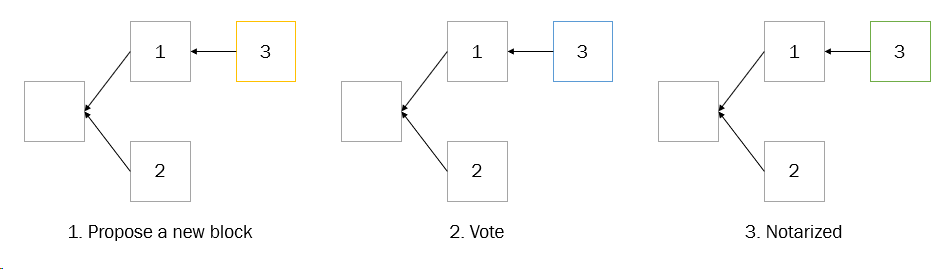
\includegraphics[width=0.7\linewidth]{Fig/15/F1}
	\caption{BFT Steps (Round-by-Round)}
	\label{fig:L15_f1}
\end{figure}
\subsection{Confirmation rule}
We call the set of distinct votes on a notarized block a \textbf{quorum certificate (QC)}.  The quorum size has to be more than two-thirds of the nodes, so that only one block per round can be notarized if the number of bad nodes is less than one-third. This is because two quorums have at least one-third of the nodes in common (see Figure 2) and only bad nodes will vote for more than one block.
\begin{figure}[h!]
	\centering
	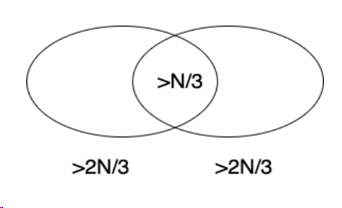
\includegraphics[width=0.25\linewidth]{Fig/15/F2}
	\caption{The intersection of two quorums must be greater than $\frac{N}{3}$.}
	\label{fig:L15_f2}
\end{figure}\\
The confirmation rule states that a block is confirmed if it has been notarized by more than two-thirds of the nodes, and if it extends a chain that has been notarized by more than one-third of the nodes.\\\\
We might think that we can confirm notarized blocks right away, since only one block per round can be notarized. But this is not secure, because there can be two blocks in different rounds that are both notarized at the same level of the blockchain, as shown by the following example.
\ex{Confirming a 1-deep notarized block is insecure.}{We cannot confirm a block just because it is notarized. Let $f$ be the number of malicious nodes, and $f<\frac{N}{3}$. In Figure \ref{fig:L15_f3}, a malicious node from round 3 makes a block $B_3$, but it only sends $B_3$ to $x$ 	honest nodes, where $\frac{2N}{3}-f < x < \frac{2N}{3}$. If all $f$ malicious nodes hide their votes on $B_3$, then no honest node will see $B_3$ as notarized. Suppose the leader of round 4 is good, then it will make a block $B_4$ at the same level as $B_3$. All good nodes vote for $B_4$, and it becomes notarized. After that, all f bad nodes show their votes on $B_3$ and make $B_3$ notarized. Since $B_3$ and $B_4$ are different (not on a chain), confirming either one of them will break safety. So notarization is not enough for confirmation.}
\begin{figure}[h!]
	\centering
	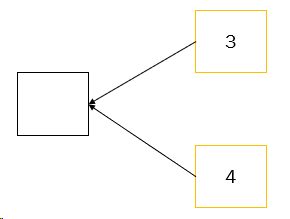
\includegraphics[width=0.2\linewidth]{Fig/15/F3}
	\caption{Conrming a 1-deep notarized block is insecure}
	\label{fig:L15_f3}
\end{figure}
Confirming a block that is k-deep in the longest notarized chain is not safe either. When the network is not fast or reliable, the adversary can create two chains that are equally long and have any length, by using the same trick as before at every level. We assume that the adversary can make any message take as long as they want when the network is slow or unreliable. In Figure \ref{fig:L15_f4}, at each level, the adversary makes sure that only $x$ honest nodes vote for the block (with an odd round number) in the upper chain, where  $\frac{2N}{3}-f < x < \frac{2N}{3}$. And after the different block (with an even round number) in the lower chain becomes notarized, the adversary shows $f$ hidden votes to make the block in the upper chain notarized. Because of this balance attack, confirming the block that is k-deep in the longest notarized chain is still not safe in Streamlet.
\begin{figure}[h!]
	\centering
	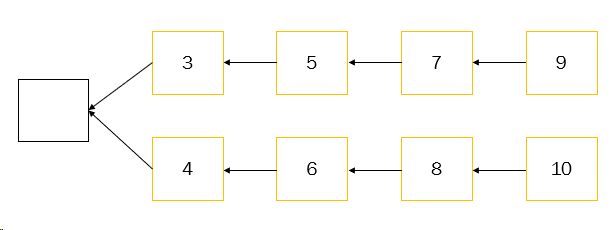
\includegraphics[width=0.5\linewidth]{Fig/15/F4}
	\caption{Confirming a k-deep notarized block is also insecure.}
	\label{fig:L15_f4}
\end{figure}\\
\textbf{Confirming a 3-deep notarized block with consecutive round numbers is secure.} The correct rule for confirming blocks in Streamlet is this: if there are three blocks next to each other in a notarized chain, and they have round numbers that go up by one, then we can confirm the chain up to the middle block of the three.\\\\
This rule is safe! Let’s say one good node sees three notarized blocks $B_5$, $B_6$, $B_7$ from rounds 5, 6, 7 in a chain (see Figure \ref{fig:L15_f5}), to show that it is safe we will argue that no other block can be notarized at the same level as $B_6$. To get a contradiction, let’s suppose there is a notarized block $B$ from round $X$ that is different from $B_6$. Because only one block per round can be notarized, we know $X$ is either bigger than 7 or smaller than 5.
\begin{itemize}
	\item  \textbf{Case 1}: $X<5$. Since block $B$ is notarized, it means that more than one-third of the honest nodes, which we call the set $S$, voted for block $B$ and also saw block $B_3$ notarized when they voted (that is, during round $X$ which is smaller than 5). Now the good nodes in $S$ will not vote for block $B_5$ in round 5, because it does not build on top of the longest notarized chain they saw, which is block $B_3$ or longer. Since $f<\frac{N}{3}$, this means that block $B_5$ can never be notarized by any good node, which is a contradiction.
	\item \textbf{Case 2}: $X>7$. Since block $B_7$ is notarized, more than one-third of the good nodes (which we call the set $S$) must have seen a notarized block $B_6$ before they voted for block $B_7$ (that is, by the end of round 7). So in round $X$ which is bigger than 7, the set $S$ of nodes must have seen block $B_6$ notarized and will not vote for block $B$, because block $B$ does not build on top of the longest notarized chain they saw (which is block B6 or longer). Since $f<\frac{N}{3}$, this means that block $B$ can never be notarized by any good node, which is a contradiction.
\end{itemize}
\begin{figure}[h!]
	\centering
	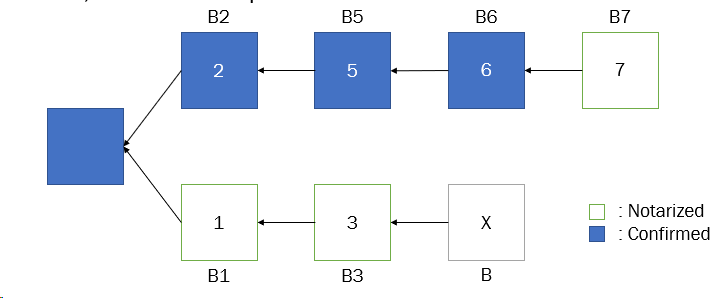
\includegraphics[width=0.5\linewidth]{Fig/15/F5}
	\caption{Streamlet confirmation example.}
	\label{fig:L15_f5}
\end{figure}

\subsection{Streamlet performance}
\textbf{Communication complexity} and \textbf{Confirmation latency} are two criteria we will discuss to measure streamlet performance. 
\subsubsection{Communication complexity of Streamlet}
Streamlet makes nodes repeat every message they get (blocks or transactions) to everyone else. Let’s say a block has $B$ bits and a vote has $V$ bits. In each round, there are $N$ senders and $N$ receivers, and on each link one block and $N$ votes are sent (because of repeating). The total communication is $N^2(B + NV) = N^2B + N^3V$ bits per block, even when the leader is good. If $N$ is big (that is, we want the protocol to work well with many nodes), $N^3V$ is the biggest part of the communication cost. Also, Streamlet needs repeating for its security (so it has to pay $N^3$ communication cost);
\ex{}{Let’s say we have a blockchain system with 7 nodes: $a, b, c, d, e, x$, and $y$. Nodes $x$ and $y$ are malicious. By round $r$, all honest nodes see the same thing. Then, $x$ is picked to be the leader of round $r$. In the first half of round $r$, it only sends its block $B$ to nodes $a, b, c$ and $y$. In the second half of the round, $a, b$ and $c$ follow the rules and vote for $B$, sending their signature to everyone. The other malicious node, $y$, only sends its vote to $a$. At this point the round is over and no more votes on $B$ are allowed. We can see that at this point a has 5 votes for $B$ (from $a, b, c, x$, and $y$), which is more than two-thirds of the nodes. But any other good node only has 4 votes for $B$. This means that only a sees $B$ as notarized. If there are no vote repeats, in the next rounds a does not vote for any block that does not build on $B$. If $a$ and $y$ stop working, the system cannot make progress. When $a$ is the leader, it tries to extend $B$ but no one else votes for it, because they don’t know it is notarized. So the chain stops growing. See Figure \ref{fig:L15_f6}}
\begin{figure}[h!]
	\centering
	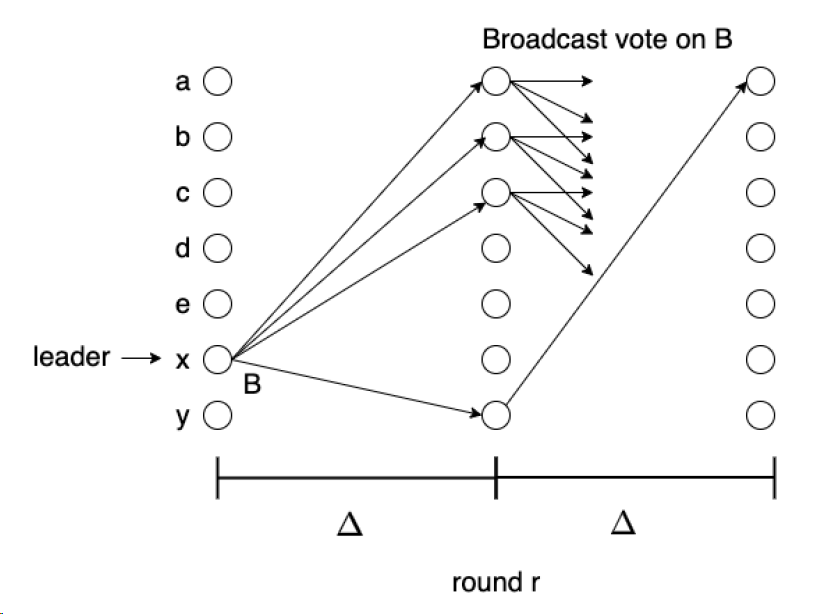
\includegraphics[width=0.5\linewidth]{Fig/15/F6}
	\caption{Communication Complexity}
	\label{fig:L15_f6}
\end{figure}
A block needs at least $N - 1$ messages to reach all nodes, so the lowest communication cost per block is $O(N)$. A blockchain protocol is linear if its communication complexity is proportional to the number of nodes. Streamlet is far from being linear because it uses broadcasting and echoing.

\subsection{Latency of Streamlet}
To guarantee liveness, Streamlet makes an assumption that rounds operate in lock-step with 2$\Delta$ duration. When there is no forking or adversary, Streamlet can confirm transactions in two rounds (or 4$\Delta$ in time). Even if there are $f < \frac{N}{3}$ malicious nodes, Streamlet can still achieve liveness as long as there are 5 honest proposers in a row. This happens on average every 7.6 rounds (or 15$\Delta$ in time), assuming that $\frac{2}{3}$ of the nodes are honest.\\\\
Recall that Bitcoin latency is $O(\ln(\frac{1}{\epsilon	})\frac{1}{\lambda\Delta})\Delta$, where $\epsilon$ is the confirmation error probability and $\lambda\Delta \ll 1$ for security. So compared to Bitcoin, Streamlet achieves much better latency: small constant and finality (i.e., deterministic confirmation).\\\\
However, BFT protocols can actually achieve even better latency by having non lock-step rounds. Streamlet sacrifices a key feature of asynchronous consensus protocols, which is responsivity. This means that the protocol can adapt to the actual network speed and not wait for the worst-case network delay. \\\\
Streamlet does not store the votes on the blockchain itself. This means that Streamlet can create a total-order on transactions, but it does not solve the problem of how an external client (who is not part of the permissioned committee) can check the validity of the ledger and confirm a transaction. This is an important issue that Streamlet does not address.

\section{HotStuff}
HotStuff is a state-of-the-art BFT consensus protocol that can achieve high performance and scalability in distributed systems. It is similar to Streamlet, but it was proposed earlier and has some advantages over it :
\begin{itemize}
	\item HotStuff is \textbf{linear}, which means that it only requires a constant number of communication steps per decision. \item It is also \textbf{responsive}, which means that it can adapt to the actual network speed and not wait for the worst-case network delay.
\end{itemize} 
HotStuff assumes that there are n nodes in the system, of which f can be Byzantine (faulty or malicious). To reach consensus, HotStuff requires a quorum certificate (QC), which is a set of 2f+1 votes on one block from different nodes. QCs are stored on the blockchain, which is a linear chain of blocks.
\begin{figure}[h!]
	\centering
	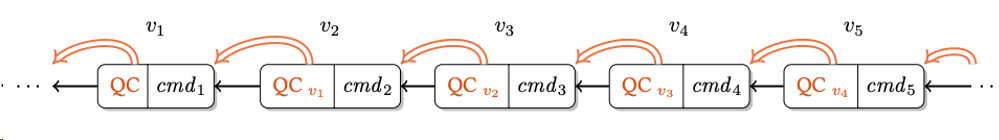
\includegraphics[width=0.7\linewidth]{Fig/15/F7}
	\caption{each node proposes a block with a command (cmd) and a QC, and how other nodes vote on it.}
	\label{fig:L15_f7}
\end{figure}\\
HotStuff uses quorum certificates (QC) to link each block to its parent block, creating a linear chain of blocks. A proposer can propose a new block as soon as it receives a new QC, without waiting for the previous block to be decided. This makes HotStuff more efficient and responsive than other protocols that require more communication steps per decision.

\subsection{From Streamlet to Hotstuff}
Every node keeps track of the QC with the highest round number (HighQC) that it knows. Like Streamlet, a proposer proposes a block that extends HighQC, and a node votes for a proposal if it follows the branch of its HighQC. However, a key difference is that a node only sends its vote to the next round’s proposer. This reduces the communication cost per block to NB + NV, where N is the number of nodes, B is the size of a block, and V is the size of a vote. Therefore, HotStuff has linear complexity, which means that it scales well with the number of nodes.\\\\
HotStuff has the same finalization rule as Streamlet: a block is finalized if it has two QCs on it and its parent, and the rounds of the three blocks are consecutive. This means that the middle block of the three blocks is irreversible (along with all the previous blocks in the chain).\\\\
HotStuff does not need round synchronization. A proposer can propose a new block as soon as it gets a new QC, which means that the protocol is driven by events rather than by time, unlike Streamlet. The protocol can advance at the speed of the actual network delays, so HotStuff is responsive. By increasing the time each node spends in each round until a decision is made, liveness is ensured.

\section{implementation: Pacemaker}
Pacemaker, which is a component that elects proposers for each round of the protocol.
The pacemaker guarantees two properties:
\begin{enumerate}
	\item eventually all nodes will be in the same round for a certain period of time
	\item there will be a unique correct proposer for that round.
\end{enumerate}
A naive way to implement the pacemaker is to double the round size until a decision is made, and to rotate the proposer among the nodes in a round-robin fashion. However, this approach has some drawbacks, such as high latency and vulnerability to network delays.

\section*{Conclusion}
Finality means that once a transaction is confirmed, it cannot be reversed or changed. Streamlet and HotStuff are two examples of such protocols, which can achieve high performance and scalability in distributed systems. They are permissioned protocols, which means that they have a fixed number of participants with known identities. They also have a strong security guarantee, which is that they can tolerate up to one-third of the nodes being faulty or malicious. However, they trade off liveness for safety, which means that they may not make progress in some situations, such as network delays or adversarial attacks.
